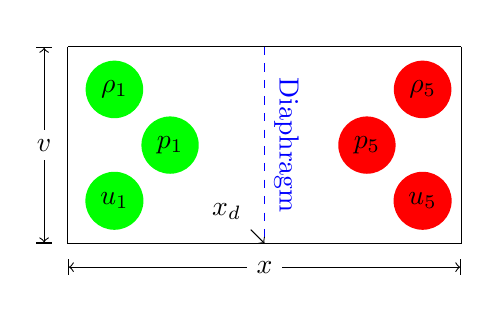
\begin{tikzpicture}
% place nodes
\node[] at (0, 0) (a) {};
\node[] at (0,-.3) (a1){};
\node[] at (-.3,0) (a2){};
\node[] at (5,0) (b) {};
\node[] at (5,-.3) (b1){};

\node[] at (0,2.5)  (c) {};
\node[] at (-.3,2.5) (c1){};
\node[] at (5,2.5) (d) {};

\node[] at (2.5,2.5)  (e) {};
\node[] at (2.5,0) (f) {};

% draw edges  
\draw[] (a.center) -- (b.center) {};
\draw[|<->|] (a1.center) -- (b1.center) node[midway,fill=white] (TextNode) {\(x\)};
\draw[] (a.center) -- (c.center) {};
\draw[|<->|] (a2.center) -- (c1.center) node[midway,fill=white] (TextNode) {\(v\)};
\draw[] (c.center) -- (d.center) node[above] {};
\draw[] (d.center) -- (b.center) node[above] {};
\draw[dashed,blue] (e.center) -- (f.center) node[sloped,above,midway] {Diaphragm};
\draw[<-] (f.center)-- +(-5pt,5pt) node[above left] {\(x_d\)};

%draw quantities
\node[circle,fill=green] at (1.3,1.25) (T){\(p_1\)};
\node [circle,fill=green,above left of=T] (rho) {\(\rho_1\)}; 
\node [circle,fill=green,below left of=T] (v) {\(u_1\)};

\node[circle,fill=red] at (3.8,1.25) (T0){\(p_5\)};
\node [circle,fill=red,above right of=T0] (rho0) {\(\rho_5\)}; 
\node [circle,fill=red,below right of=T0] (v0) {\(u_5\)};
\end{tikzpicture}